\documentclass[twocolumn]{article}
\usepackage[portuguese]{babel}
\usepackage[utf8]{inputenc}
\usepackage{graphicx}

\title{Sokoban}
\author{
  Filipa Correia
  \and
  Nuno Maia
}
\date{Maio 2014}

\begin{document}

\maketitle

\begin{abstract}
Este estudo descreve os diferentes métodos usados para a resolução de puzzles Sokoban, as suas vantagens e desvantagens...
\end{abstract}

\section{Introdução}
O Sokoban parece, à partida, um jogo relativamente simples. No entanto, as abordagens tomadas inicialmente continuavam a ser insuficientes para a resolução de alguns puzzles. Sendo assim, fomos incrementalmente alterando ou adicionando novas funcionlidades. Neste estudo, fazemos uma breve descrição do jogo e apresentamos todos os passos relevantes deste processo e valores significativos que permitem distinguir as várias abordagens.

\section{Sokoban}

O Sokoban é um jogo cujo objectivo é empurrar as diversas caixas, espalhadas num dado espaço, para os seus destinos evitando os obstáculos que aparecem à sua frente. Nós, humanos, conseguimos resolver estes problemas com alguma facilidade mas fazer com que um computador consiga resolvê-lo por nós implica um grande esforço devido ao grande espaço de estados gerados.

\begin{figure}[ht!]
\centering
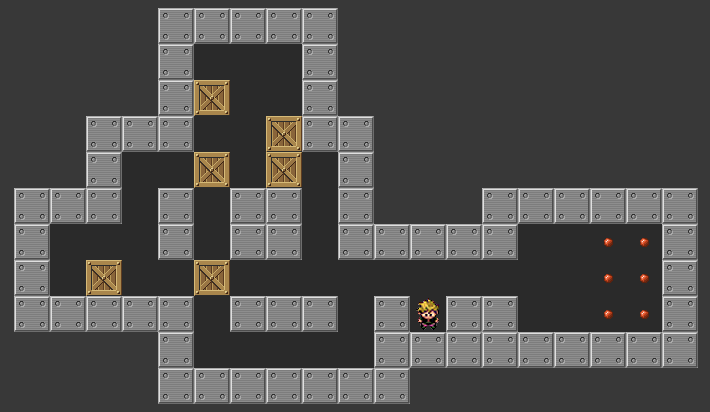
\includegraphics[width=0.4\textwidth]{sokoban.png}
\caption{Primeiro puzzle original}
\end{figure}

\section{Modelação do problema}

O Sokoban tem regras muito simples. O jogo é composto por apenas quatro elementos distintos: o homem, as caixas, os destinos e as paredes. Ainda podemos considerar o homem e as caixas numa posição de destino. O homem só pode efectuar quatro tipos de movimentos (pode deslocar-se para cima, baixo, esquerda ou direita). Para conseguirmos ter uma percepção de qual a maneira mais adequada para resolver os diferentes puzzles que compõem o jogo, foram implementadas duas formas distintas de o fazer: pushing e pulling.

\subsection{Pushing}

Esta trata-se da modelação normal deste problema. O homem, quando se encontra numa posição adjacente a uma caixa, tem que decidir se consegue ou não empurrar a caixa. De modo a que o movimento da caixa seja considerado como proveitoso, tem que ser feitas algumas verificações como se a próxima posição de caixa é um canto, se vai impedir que outras caixas ou ela própria se possam movimentar. Estas verificações serão detalhadas mais à frente.

\subsection{Pulling}

A segunda modelação deste problema consiste na inversão do objectivo do jogo, isto é, em vez de o objectivo ser colocar as caixas nos destinos, passamos a considerar que os destinos são as posições originais das caixas e que as caixas começam colocadas nas posições de destino. Assim, o homem não precisa de empurrar caixas mas sim puxá-las. Esta alternativa ao modo de resolver o problema permite evitar alguns dos problemas que a modelação original trás.

\section{Estruturas de dados}

Para a resolução deste problema, tivémos que pensar quais seriam as estruturas de dados mais adequadas para manter a sua manipulação o mais simples possível e, consequentemente, que não ocupasse demasiada memória. Existem duas estruturas de dados principais na nossa implementação: o mapa e a representação do estado.

\subsection{Mapa}

O mapa é representado por uma estrutura que mantém a informação necessária sobre o mesmo. É composto por um array que guarda as posições de todas as paredes, outro array que serve como auxiliar para poderem ser colocadas as caixas, de maneira que a se consiga ter uma percepção de onde é que elas se situam, uma lista de posições de destino e ainda as dimensões do mesmo.

\subsection{Estado}

Esta estrutura é usada em todas as procuras para representar a situação atual da execução. Dado o elevado número de estados gerados na resolução dos puzzles, é importante que a representação do estado seja o mais simples possível, de modo a limitar o espaço de memória necessário para o guardar. Assim, o nosso estado é representado apenas por uma lista. Esta lista guarda apenas as posições atuais das caixas e o caminho percorrido pelo homem até ao momento. Anteriormente, este era composto também pelo mapa mas chegámos à conclusão que não havia necessidade de manter esta estrutura em todos os estados visto que o mapa não muda ao longo da execução. Assim, mantemos o mapa guardado numa variável global de forma a poder ser usado em qualquer ponto da execução.

\section{Heurísticas}

\section{Estratégias de corte}

Como já foi referido anteriormente, a resolução dos puzzles Sokoban implicam a geração de um elevado número de estados. O problema é que nem todos os estados gerados resultam em movimentações de caixas que interessam para atingir a solução. Existem algumas situações que sabemos de antemão que devemos evitar ou em que podemos aplicar mais de que uma operação possível.

\subsection{Cantos}

Os cantos são formados por qualquer combinação de três paredes ou caixas. Uma caixa colocada nestas posições, nunca vai poder ser retirada da mesma, logo, temos que arranjar uma maneira de evitar que isso aconteça. \\
Para detectar estes cantos na modelação do problema em que o homem empurra as caixas, decidimos adicionar informação ao mapa que indicasse que posições constituiam cantos. Assim, na geração de sucessores, se a próxima posição da caixa for um canto, podemos descartar esse sucessor. \\
Já na modelação do problema em que o homem puxa as caixas, não precisamos de fazer qualquer verificação porque, para uma caixa poder ficar num canto, o homem teria que ocupar uma posição que estaria ocupada com uma parede ou com uma caixa e isso nunca pode acontecer.

\subsection{Freeze Deadlocks}

\subsection{Túneis}


\section{Resultados}

\section{Conclusões}

\end{document}
